\documentclass{article}
\usepackage[utf8]{inputenc}
\usepackage{indentfirst, graphicx, wrapfig, amsmath}
\usepackage[margin=1.0in]{geometry}
\usepackage[backend=biber]{biblatex}
\addbibresource{bib.bib}


\begin{document}

\begin{center}
\huge{{2-Dimensional Metaballs}}\\
\huge{{Michael Chen \& Douglass Boshkoff}}\\
\huge{{December 16 2016}}
\end{center}

\section*{Introduction}

Metaballs are amorphous, fluid surfaces that combine and separate smoothly. For our project, we chose to implement two dimensional metaballs. In this report, we will go over our how metaballs are drawn, our implementation process, and possible extensions on this project. 

\subsection*{Compilation \& Options}

To run our program you just need to compile using make and run the \emph{final} executable. Once the program is running, use \emph{M} to toggle between the drawing modes  that we have implemented. You can also use \emph{S} and \emph{Shift + S} to stop and re-start the program respectively.

\section*{Metaballs Implementation}

To create metaballs, we needed to first draw circles that bounce off the edges of the predetermined x and y boundaries. We defined the drawing plane to be -100 to 100 in both the x and y directions. We use ten circles that move in random directions with random radii to model our metaballs. After we succeeded in drawing all of our circles and got the circles to bounce correctly, we moved onto implementing the marching squares algorithm which is responsible for efficiently calculating a smooth approximation of the metaball boundary. To implement the marching squares, we first needed to create a sampling grid of the drawing plane. This grid consisted of a 51 by 51 two dimensional array that would define the four corners of every square to be used in the marching squares algorithm. The reason we used a 51 by 51 two dimensional array is so we could divide the drawing plane into 2500 equally sized squares. 

Once we partitioned our drawing plane, we then needed to calculate the contribution from every circle to every point in the sampling grid. To calculate the contributions we used a thresholding function based on the equation of a circle where x and y can be any point within the sampling grid

\begin{equation*}
\frac{r^2}{(x - x_0)^2 + (y - y_0)^2} \geq 1 
\end{equation*}
This equation defines points that are inside the circle. However, we want to consider all of the circles, rather than just one circle. For this reason we use the summation of the contributions of all of the circles. Thus, we define our thresholding function as follows. 

\begin{equation*}
f(x,y)=\sum_{i = 0}^{n} \frac{r_i^2}{(x - x_i)^2 + (y - y_i)^2}
\end{equation*}

If $f(x,y)$ is greater than one we say that point $(x,y)$ is above the threshold. This means, that the point is inside a metaball.

This thresholding function defines the metaballs in terms of the sampling grid. When two circles draw close together their contributions create a bridging effect between the metaballs. While this provides a good starting point for drawing metaballs, it results in a fairly blocky and uninteresting visual effect. We could increase the resolution of the sampling grid, but this would make the algorithm incredibly computationally intensive. Instead, we can use marching squares to interpolate points within each square of our sampling grid to generate smooth contour lines for the metaballs. 

\subsection*{Marching Squares}
The basic idea behind the marching squares algorithm is that we can determine information about the metaballs boundary by the knowledge of which vertices are above our threshold value. Within each square, there are four vertices each of which can either be above or below threshold. When we one vertex is above the threshold and another adjacent vertex is below threshold, we know that the edge of a metaball goes through the edge between those two vertices. Using linear interpolation we can approximate where the metaball intersects the edge.  Figure 1 shows a few possible shapes that can be drawn with a square where the green vertices are above threshold and the white vertices are above threshold.



\section*{Our Design}
\begin{wrapfigure}{R}{.085\textwidth}
\begin{center}
    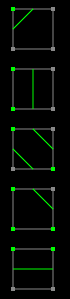
\includegraphics[scale = 0.5]{msquares2}
    \caption{from \cite{Wong}}
\end{center}
\end{wrapfigure}
We use Qt and opengl to implement this project. Most of our important code is either in mypanelopengl or in the circle class. Each circle has a randomly generated velocity, radius, and color. Each circle has its own VBO and VAO which are used in its draw function. 

In mypanelopengl, most of the pertinent code is inside the call to paintGl which is called every 20 milliseconds. On every call to paintGl, we calculate the threshold values for the sampling grid. We conceptualize the drawing as taking place separately for each square of the 2500. So the main issue becomes how to draw the shape created by the interpolated points, if there are any, along with the vertices above the threshold. To do this we first generate all the vertices in the triangles. We use the following algorithm find the vertices of the triangles in each square.

Start with the lower right corner of the square. If the lower right corner is above threshold check the upper right corner. If both of corners are above threshold, insert both into the list of vertices. Otherwise insert the lower right vertex and the point interpolated between the lower right vertex and upper right vertex into the list. Repeat this algorithm for every other vertex in the square. 

Now we have a list of the vertices which define the shape in each square. With this list we can fill out the local VBO in mypanelopengl to draw triangles using the GL\_TRIANGLE primitive. By drawing the shapes within each square we can construct each metaball smoothly without huge amounts computations. 

\subsection*{Screencaps}


\begin{figure}[h]
\centering
\begin{minipage}{.5\textwidth}
  \centering
  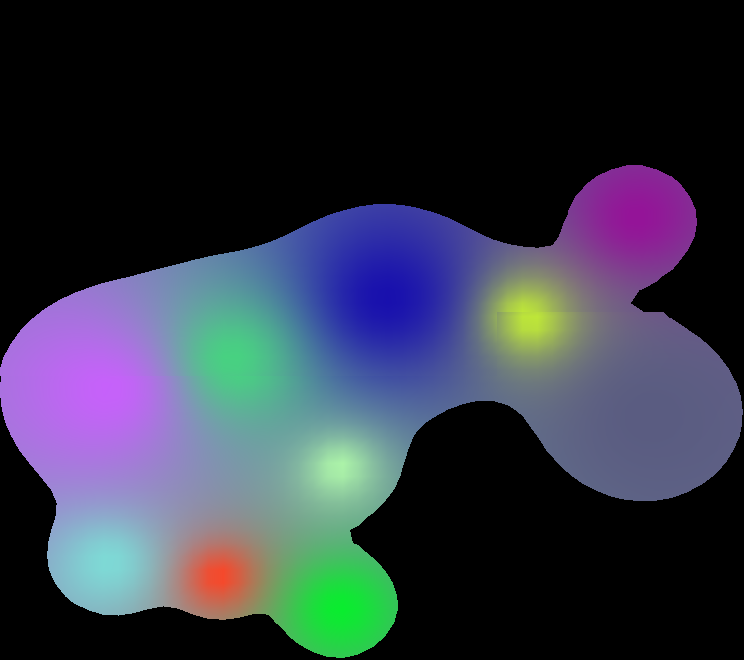
\includegraphics[width=0.7\textwidth]{colormeatballs}
  \caption{Meatballs with blended colors}
\end{minipage}%
\begin{minipage}{.5\textwidth}
  \centering
  
\includegraphics[width=0.7\textwidth]{metaballs}
  \caption{Regular meatballs with a magenta color}
\end{minipage}
\end{figure}


\section*{Goals and Further Work}
Our original goal was to implement two dimensional metaballs then port our program to three dimensions. We thought that it would be fairly simple to change from two dimensions to three dimensions. However, we realized that some of our algorithms would need to be drastically reconstructed to convert to three dimensions. So, we decided not to move to three dimensions. 

Instead, we decided to write another vertex shader that would take in a separate color value for each vertex. We calculated these color values by giving each circle its own random color, and blending these colors depending on the amount the circle contributed to the total contribution value for each point in our sampling grid. This created an interesting blending effect for the metaballs. 

If we were to keep working on this project, we would choose to reconstruct out algorithms to convert to three dimensions and implement Phong lighting. We would also like to add a physics library to simulate a lava lamp using the metaballs program. 

\printbibliography

\begin{figure}[h]
\begin{center}
    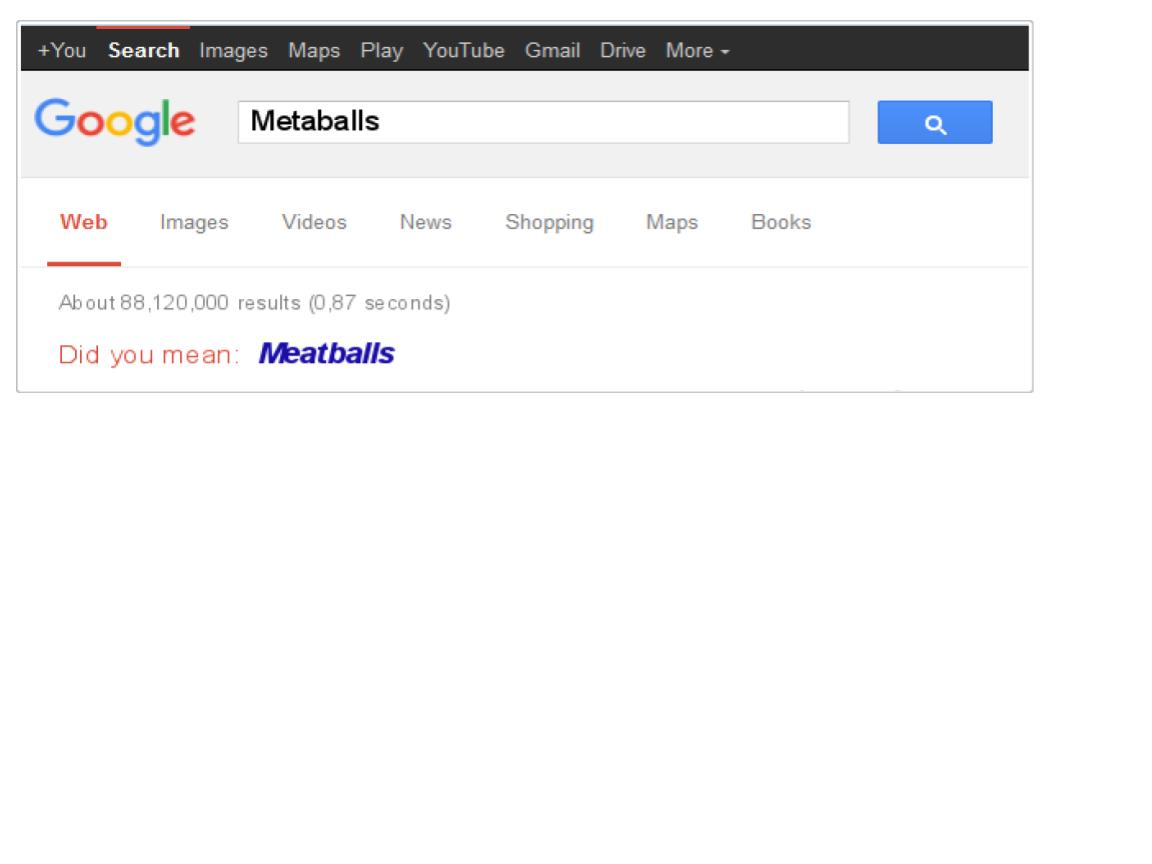
\includegraphics[scale=0.3]{DidYouMean?}
\end{center}
\end{figure}
\end{document}
